%-----------------------------------------------------
\begin{frame}[allowframebreaks,fragile]{TEI for Digital Editing}

\subsection{TEI elements relevant to editing}
\metroset{block=fill}\small

\begin{columns}
\column{0.3\textwidth}
TEI can describe the structure of a text, e.g.
\begin{itemize}
\item  speaker, verse line, stage directives
\item  greeting, signature
\item  Visual aspects of the script
\item  special characters, new lines
\end{itemize}

\begin{xmlcode}
<fw place="top-centre" type="head">Poëms.</fw>
<fw place="top-right" type="page-no">29</fw>
\end{xmlcode}

\column{0.68\textwidth}\vspace{-3em}
\begin{block}{Simple layout markup}\footnotesize
\begin{itemize}
\item  beginning of a new \textbf{line}: \texttt{<lb/>}
\item  beginning of a new \textbf{page}: \texttt{<pb/>} \texttt{@n} for an explicit numbering
\item  beginning of a new \textbf{column}: \texttt{<cb/>}
\item  \textbf{highlighted} text: \texttt{<hi>}
\begin{itemize}\scriptsize
    \item Attribute \texttt{@rend} to describe the appearance
    \item Alternative encoding: \emph{<foreign>}, \emph{<emph>}, \emph{<distinct>}
\end{itemize}
\item  graphical elements in the text: \texttt{<figure>}
\item  \texttt{<fw>} (forme work) contains a running head (e.g.
a header, footer), \textbf{catchword}, or similar material
appearing on the current page.
\end{itemize}
\end{block}
\end{columns}


\framebreak

\begin{columns}
\column{0.48\textwidth}
\begin{alertblock}{Documenting particularities of the writing surface}\scriptsize
\begin{description}
\item[<damage>] \texttt{@agent, @degree, @unit, @quantity, @extent, @precision, @scope}
\item[<unclear>]
\item[<gap>] any ommission in the transcription -- @reason, e.g. sampling, inaudible, irrelevant, cancelled
\end{description}
\end{alertblock}


\includegraphics[width=0.5\textwidth]{img/tei-unclear.png}
\vspace{2em}

\begin{xmlcode}
<gap reason=“wormhole" quantity="5" unit="character"/>
<damage agent=“coffee” quantity=“3” unit=“line”/>
\end{xmlcode}

\column{0.5\textwidth}
\begin{alertblock}{Other important attributes}
\begin{description}\scriptsize
    \item[@cert(ainty)] how certain you are about the suggested transcription?
    \item[@resp(onsibility)] who did it?
    \item[@evidence] where you got the clues from (internal, external, conjecture)?
\end{description}
\end{alertblock}

\begin{xmlcode}
I <subst>
 <add place="above">might</add>
  <del>
   <unclear reason="overinking"
      cert="medium" resp="#LDB"> 
      should</unclear>
  </del> </subst> have
\end{xmlcode}
\end{columns}


\end{frame}

%-----------------------------------------------------
\begin{frame}[allowframebreaks,fragile]{Transcription}
\subsubsection{Transcription}
\metroset{block=fill}

\begin{columns}
\column{0.48\textwidth}
\begin{itemize}\small
\item  OCR (Optical Character Recognition) -- e.g. Transkribus (transcription support)
\item  also:  Transkribus Keyword Spotting 
\item  also:  fuzzy search which should also find the word if it's mistranscribed
\item  Writer identification
\end{itemize}

\column{0.48\textwidth}

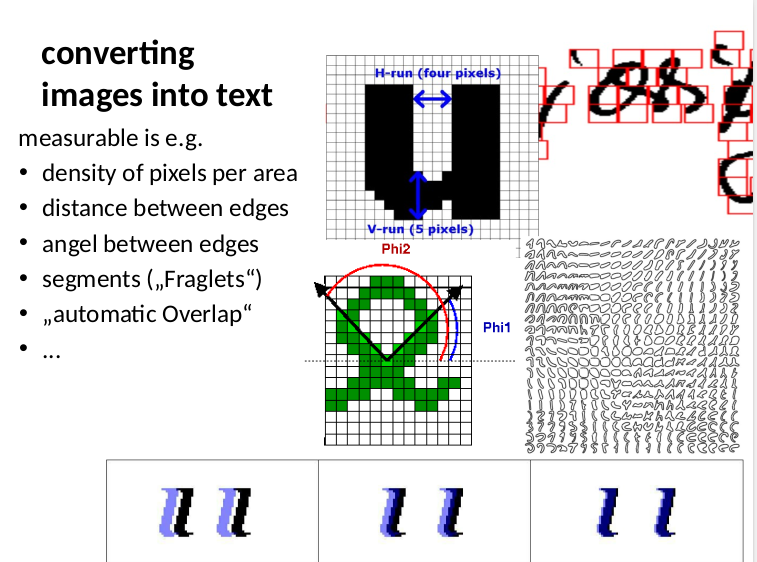
\includegraphics[width=\textwidth]{img/ocr1.png}
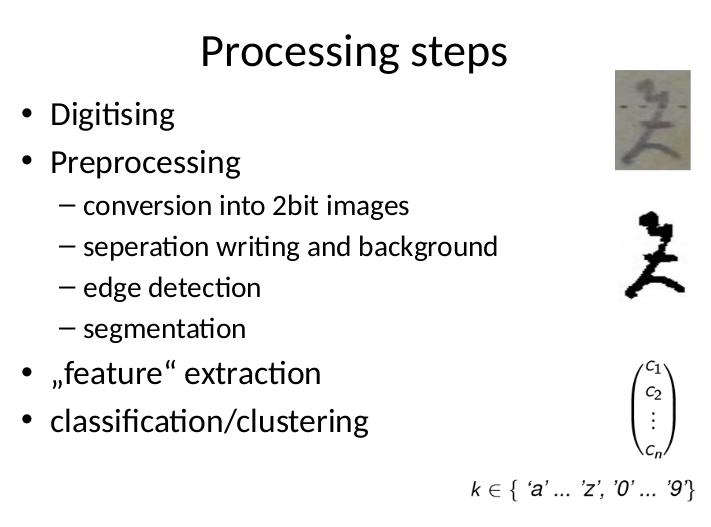
\includegraphics[width=\textwidth]{img/ocr2.png}
\end{columns}

\framebreak 

\begin{columns}
\column{0.48\textwidth}
\begin{block}{Typical phenomena}
\begin{itemize}
\item “Special characters"
\item Abbreviations
\item damaged or unreadable text
\item additions, deletions, substitutions, corrections
\item editorial interventions (emendations and conjectures)
\item  editorial additions or omissions
\end{itemize}
\end{block}

\column{0.48\textwidth}

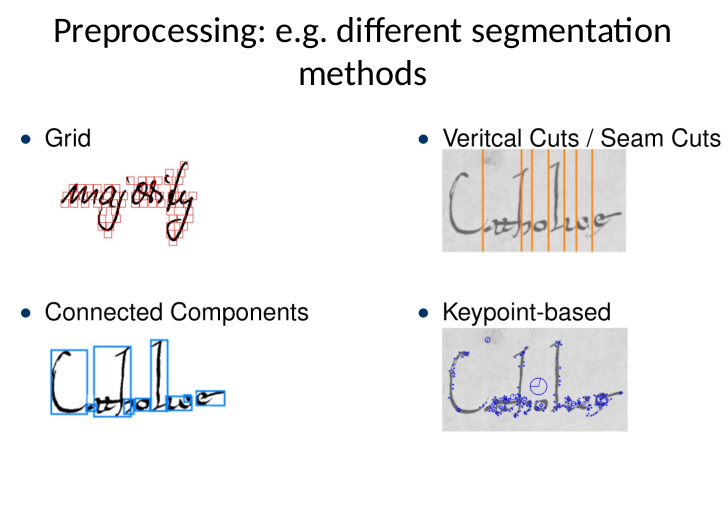
\includegraphics[width=\textwidth]{img/ocr3.png}
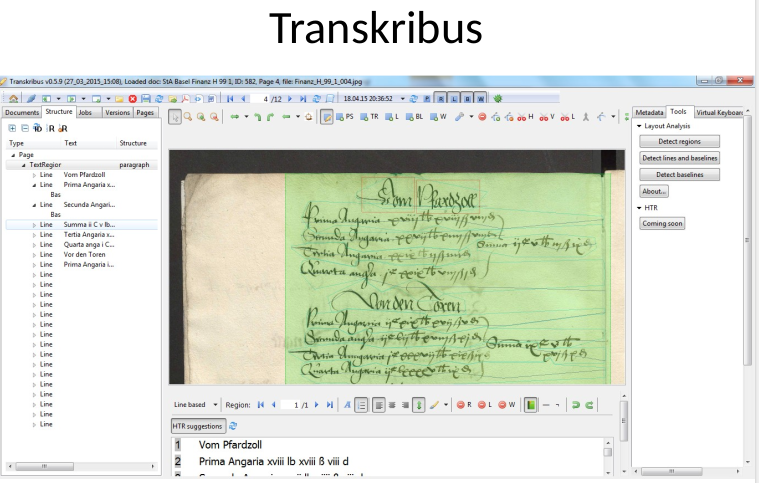
\includegraphics[width=\textwidth]{img/ocr4-transkribus-app.png}

\end{columns}

\framebreak

Transcriptions contain: 
\begin{columns}
\column{0.4\textwidth}
\begin{itemize}
\item  layout
\item  additions
\item  corrections
\item  modifications
\item  voids, space, holes, gaps \dots
\item  alternative transcriptions
\item  editorial interventions
\item  Enhanced transcription
\end{itemize}

\column{0.55\textwidth}
\begin{xmlcode}
<pb>, <lb>, <cb>, <hi>, <g>, 
<handShift/>
<add>, <addSpan>,
<corr>, <del>, <delSpan>, <sic>
<subst>
<gap>, <damage>
<choice>, <alt>
<unclear>, <supplied>, <reg>
<add>, <addSpan>, <corr>, <choice>, 
<damage>, <del>, <delSpan>, 
<restore>, <gap>, <sic>
\end{xmlcode}
\end{columns}

\end{frame}


%-----------------------------------------------------
\begin{frame}[fragile]{Genetic Edition}
\metroset{block=fill}

\begin{columns}
\column{0.48\textwidth}
\begin{block}{Critique Génétique}\footnotesize
\textbf{Research interest:} Reconstruct the writing process in the working manuscripts of the author
\end{block}

\column{0.48\textwidth}
\begin{xmlcode}
That's <del xml:id="del1">
superfluous 
<restore>
 <redo target="del2" /> 
 <del xml:id="del2">deleted</del> 
</restore> </del>
text.
\end{xmlcode}
\end{columns}



\begin{columns}
\column{0.48\textwidth}
\begin{xmlcode}
<zone>
 <line>Alone
  <seg type="alternative" 
   xml:id="alt1"> before </seg>
  <add place="above" 
       type="alternative"
       xml:id="alt2">beside</add> 
  his native river—
 </line>
 <alt targets="#alt1 #alt2" 
      mode="excl" weights="01"/>
</zone>
\end{xmlcode}
\column{0.48\textwidth}
\begin{xmlcode}
He sat <seg type="transposition" 
xml:id="trans1"> at
his table</seg> 
<seg type="transposition"
xml:id="trans2"> head on hands
</seg>.

<listTranspose>
<transpose>
  <ptr target="#trans2"/>
  <ptr target="#trans1"/>
</transpose>
</listTranspose>
\end{xmlcode}
\end{columns}

\end{frame}


%-----------------------------------------------------
\begin{frame}[fragile]{The script: palaeography}
\metroset{block=fill}

\begin{columns}
\column{0.58\textwidth}
\begin{itemize}
\item  soft hyphen: \texttt{@break=“no”}
\item  \texttt{@rend | @rendition}
\begin{itemize}
    \item \texttt{@rend}: verbal description; each word describes a single facet (\texttt{rend=“indented:5cm”})
    \item \texttt{@rendition}: reference to description of the rendition in the \texttt{teiHeader//encodingProfile}
\end{itemize}
\item  „special characters":
\begin{itemize}
    \item \texttt{<g>}
    \item Does it exist in Unicode? (\protect\url{http://www.unicode.org}). As an entity in XML:
\begin{xmlcode}
&#x[hexadecimal code];
&#[decimal code];
\end{xmlcode}
\end{itemize}
\end{itemize}

\column{0.38\textwidth}
\begin{block}{Unicodefor historical texts}\scriptsize
\begin{itemize}
\item  \emph{Combining Diacritical Marks} (0300–036F) and \emph{Supplement} (1DC0–1DFF): Superscripts, Subscripts
\item  \emph{Latin Extended Additional} (1E00–1EFF): characters with diacritics
\item  \emph{Latin Extended-D} (A720–A7FF): Ligatures, abbreviations, \dots
\item  \emph{General Punctuation} (2000–206F) and \emph{Supplement} (2E00–2E7F)%: \#\#Hochpunkte etc.
\item  \emph{Ancient Symbols} (10190–101CF): roman measurements, coins\dots
\end{itemize}
\end{block}
\end{columns}


\end{frame}
%-----------------------------------------------------
\begin{frame}[fragile]{Editorial interventions}
\metroset{block=fill}

\begin{columns}
\column{0.48\textwidth}
\begin{itemize}
    \item expansion of abbreviations
    \item Conjectures
    \item Normalisations
\end{itemize}
\column{0.48\textwidth}
\begin{itemize}
\item \texttt{<abbr>, <expan>} plus \texttt{<am>, <ex>}
\item \texttt{<sic>, <corr>}
\item \texttt{<orig>, <reg>}
\end{itemize}
\end{columns}\bigskip

\begin{block}{All these can be paired:}
\begin{itemize}
    \item General for all editorial interventions: \texttt{<choice>}.
    \item Explicitly for substitutions: \texttt{<subst>}.
    \item \texttt{<supplied>} for additions by the editor
    \item \texttt{<unclear>} for unreadable text (\texttt{@reason, @agent, @hand})
\end{itemize}
\end{block}

\end{frame}
%-----------------------------------------------------
\begin{frame}[allowframebreaks,fragile]{Abbreviations}
\metroset{block=fill}\small 

\begin{columns}
\column{0.42\textwidth}
In Western MS, we usually distinguish:
\begin{itemize}\scriptsize
\item  \textbf{Suspensions:} the first letter or letters of the word are written, generally followed by a point : for example ‘e.g.’ for ‘exempla gratia’
\item  \textbf{Contractions:} both first and last letters are written, generally with some mark of abbreviation such as superscript strokes, or points : e.g. ‘Mr.’ for ‘Mister’
\item  \textbf{Brevigraphs:} Special signs such as the Tironian nota used for ‘et’, the letter p with a barred tail used for ‘per’, the letter c with a circumflex used for ‘cum’/’con’ etc.
\item  \textbf{Superscripts:} Superscript letters (vowels or consonants) used to indicate various kinds of contraction: e.g. ‘w’ followed by superscript ‘ch’ for ‘which’.
\end{itemize}

\column{0.56\textwidth}
\begin{itemize}\small 
\item  \texttt{<expan>} The element content is considered as the expansion of an abbreviation. In the text: USA $\to$ transcription: 
\begin{xmlcode}
<expan>United States of America</expan>
\end{xmlcode}
\item  \texttt{<abbr>} The element content is an abbreviation
\begin{xmlcode}
<abbr>USA</abbr>
\end{xmlcode}
\item  \texttt{<ex>} (expansion) and \texttt{<am>} (abbreviation mark) for the  omitted part of the abbreviation, e.g.
\begin{xmlcode}
e<ex>xempla</ex> g<ex>ratia</ex>
e<am>.</am> g<am>.</am>
\end{xmlcode}
\end{itemize}
\end{columns}

\framebreak

Abbreviations can also be considered as alternatives: \texttt{<choice>}, e.g. `Zum Beispiel' and `z.B.':
\begin{xmlcode}
<choice>
 <expan>Zum Beispiel</expan>
 <abbr>Z.B.</abbr>
</choice>
\end{xmlcode}

Or respectively:
 \begin{xmlcode}
Z<choice>
   <am>.</am>
   <ex>um</ex>
  </choice>
  
B<choice>
   <am>.</am>
   <ex>eispiel</ex>
 </choice>
\end{xmlcode}


\end{frame}

%----------------------------

\begin{frame}{Transcription = Interpretation}
\metroset{block=fill}\small

\begin{columns}
\column{0.48\textwidth}\small
`gemination dash' – possible solutions:
\begin{itemize}\footnotesize
\item  Uncommented expansion
\item  Unicode m with "combining macron"
\item  Encoding as an XML-Entity
\item  \texttt{<g>} refering to \texttt{<charDecl>}
\item  Only \texttt{<am/>} for the stroke
\item  Only \texttt{<ex>} for the expansion
\item  As a \texttt{<choice>} with \texttt{<abbr>} and \texttt{<expan>}, the first incl.
a abbreviation mark \texttt{<am>} and the second the
expansion \texttt{<ex>}
\end{itemize}

\begin{block}{Gemination dash}\scriptsize
horizontal, bended or curved stroke above a nasal letter indicating the omission of a further instance of the same letter.~(\href{https://www.degruyter.com/database/WSK/entry/wsk_id_wsk_artikel_artikel_14933/html?lang=en}{source})
\end{block}

\column{0.48\textwidth}
\begin{block}{Modifications}\footnotesize
\begin{itemize}
\item  addition, deletion, substitution, transpose, \emph{or:}
\item  modification (represents any kind of general
modification without interpretation)
\end{itemize}
\end{block}

\begin{alertblock}{Changing writer}\footnotesize
\begin{description}
\item[<handShift />] \texttt{@new} : the hand which writes from this place onward
\item[<handDesc>] (part of \texttt{msDesc}) 
\item[<handNotes>] (part of \texttt{profileDesc})
\item[<handNote>] for a particular description
\item[@xml:id] an identifier for the hand
\end{description}
\end{alertblock}
\end{columns}


\end{frame}

%-----------------------------------------------------
\begin{frame}[allowframebreaks,fragile]{Text and images}
\subsubsection{Text and images}

\metroset{block=fill}
\begin{columns}
\column{0.4\textwidth}
Images of a text are encoded in a \texttt{facsimile} --
structure parallel to \texttt{teiHeader} and \texttt{text}:
\begin{xmlcode}
<tei>
  <teiHeader>...</teiHeader>
  <facsimile> ...</facsimile>
  <text>...</text>
</tei>
\end{xmlcode}

\column{0.58\textwidth}
\begin{alertblock}{\texttt{<facsimile>}}\footnotesize
\begin{itemize}
\item  \texttt{<surface>} = something meant to be seen
\begin{itemize}
    \item \texttt{@uly, @ulx; @lrx, @lry} =upper left x/y- and lower right y/x coordinates
    \item  coordinates form a grid, which can be referred $\to$ \texttt{@ulx} and \texttt{@uly} are usually 0
\end{itemize}
    \item \texttt{<graphic>}: image, \texttt{@url} : image file
     \item  \texttt{<zone>} = an area on the surface. Coordinates refer to the grid defined in \texttt{@uly}, \texttt{@ulx}; \texttt{@lrx, @lry} of the \texttt{<surface>}.
\end{itemize}
\end{alertblock}
\end{columns}


\framebreak

\begin{columns}
\column{0.48\textwidth}
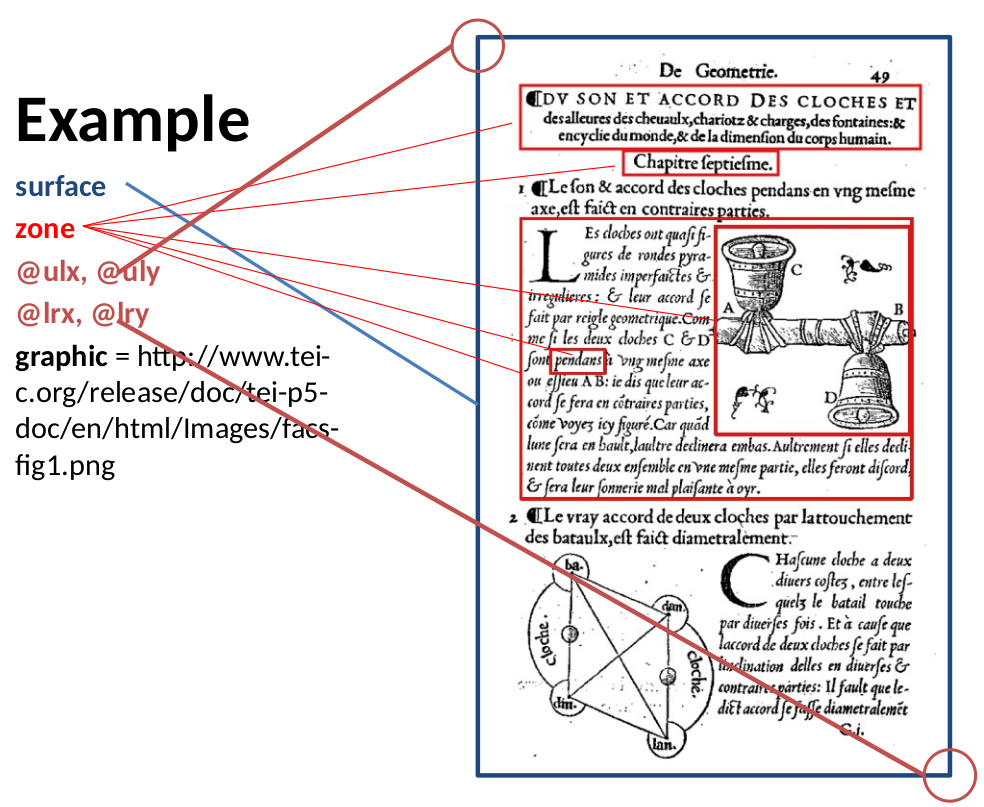
\includegraphics[width=\textwidth]{img/facs1.png}
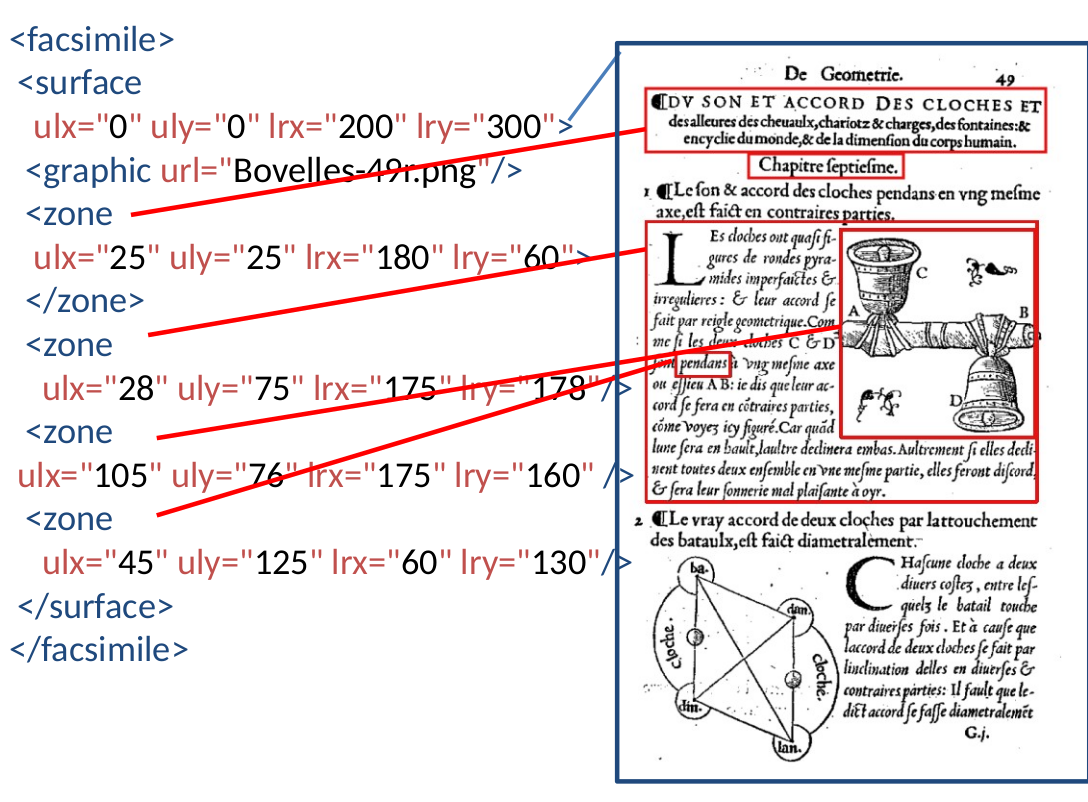
\includegraphics[width=\textwidth]{img/facs2.png}
\column{0.48\textwidth}
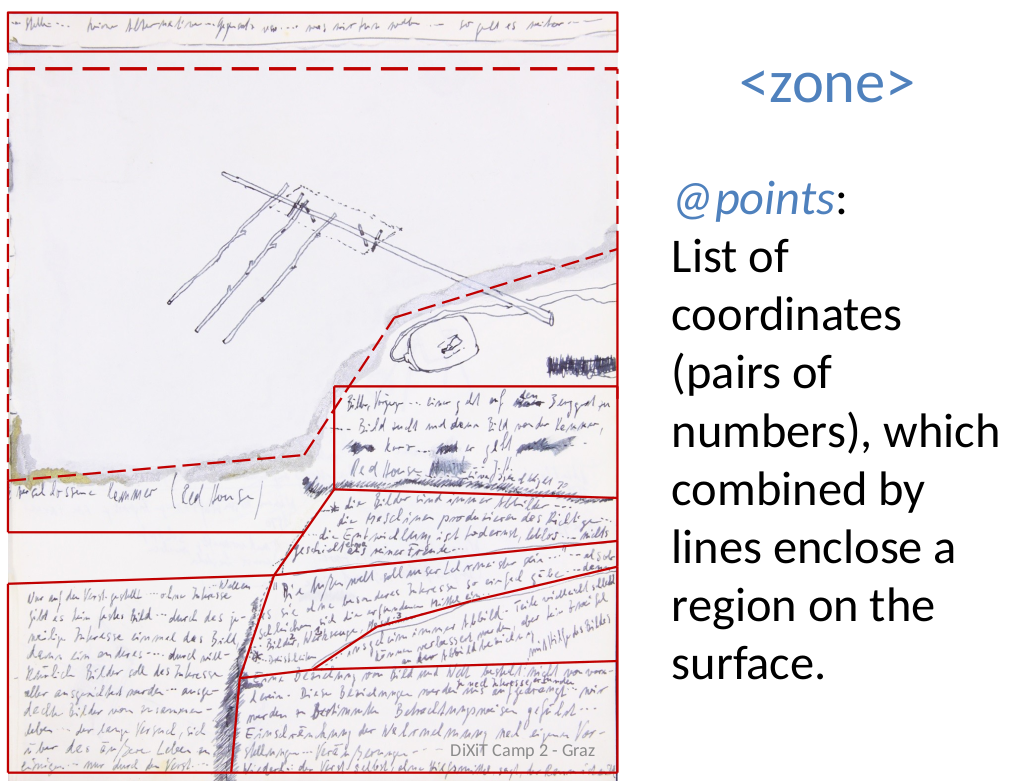
\includegraphics[width=\textwidth]{img/facs3.png}
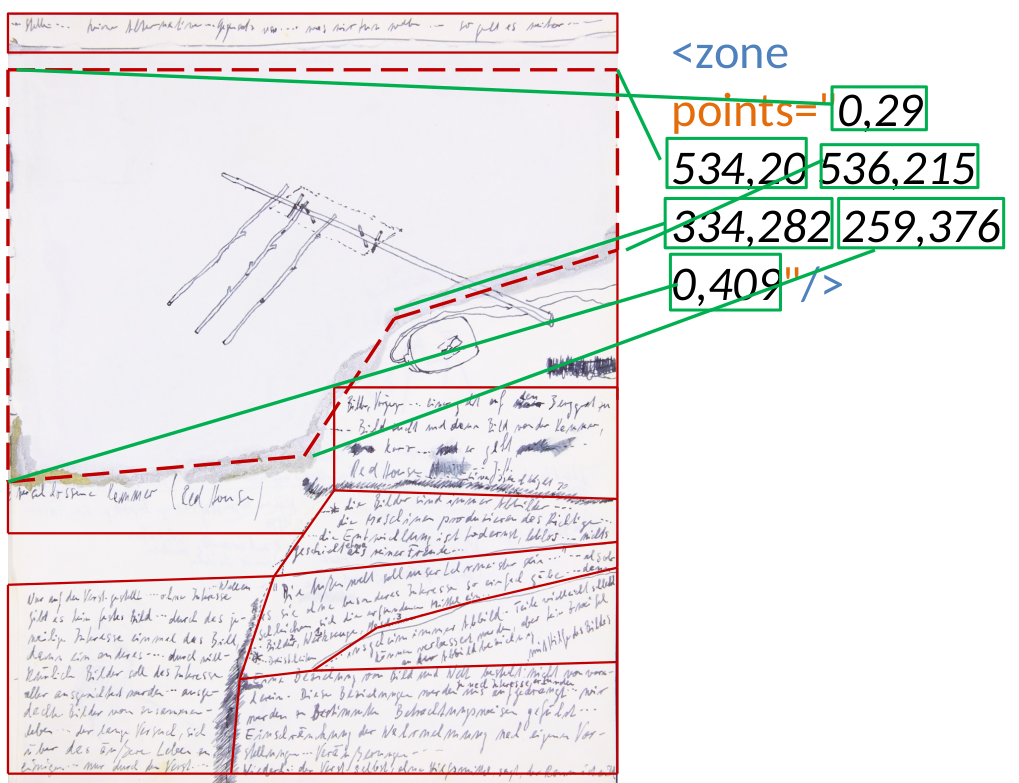
\includegraphics[width=\textwidth]{img/facs4.png}
\end{columns}

\framebreak

\begin{columns}
\column{0.48\textwidth}

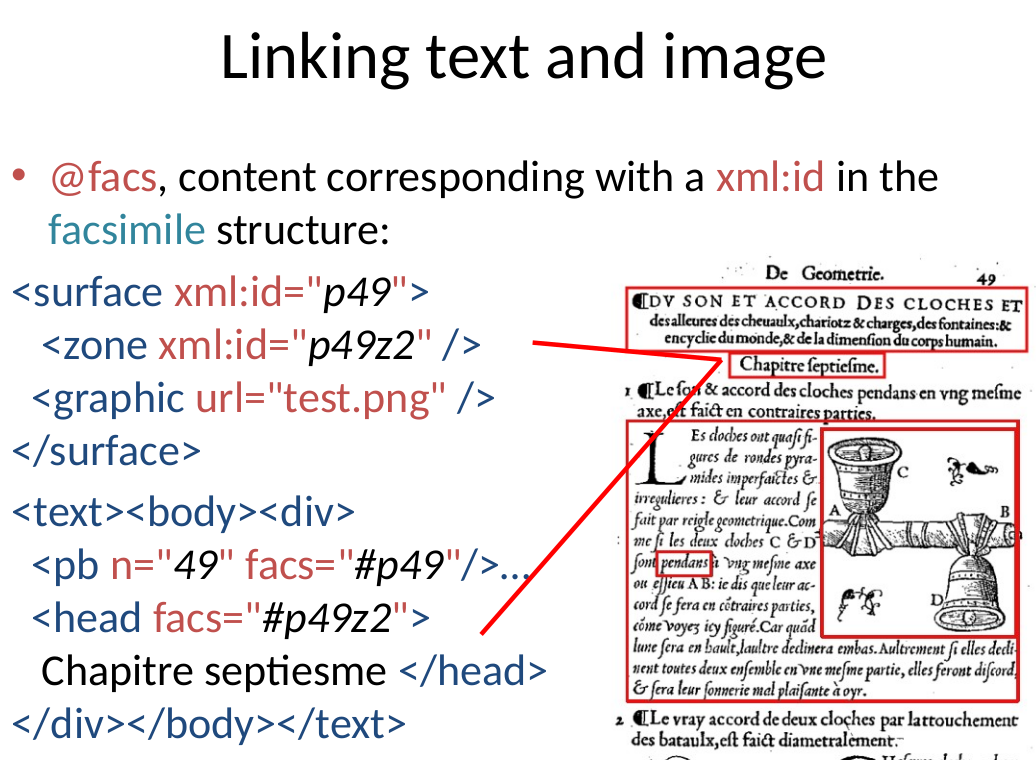
\includegraphics[width=\textwidth]{img/facs5.png}
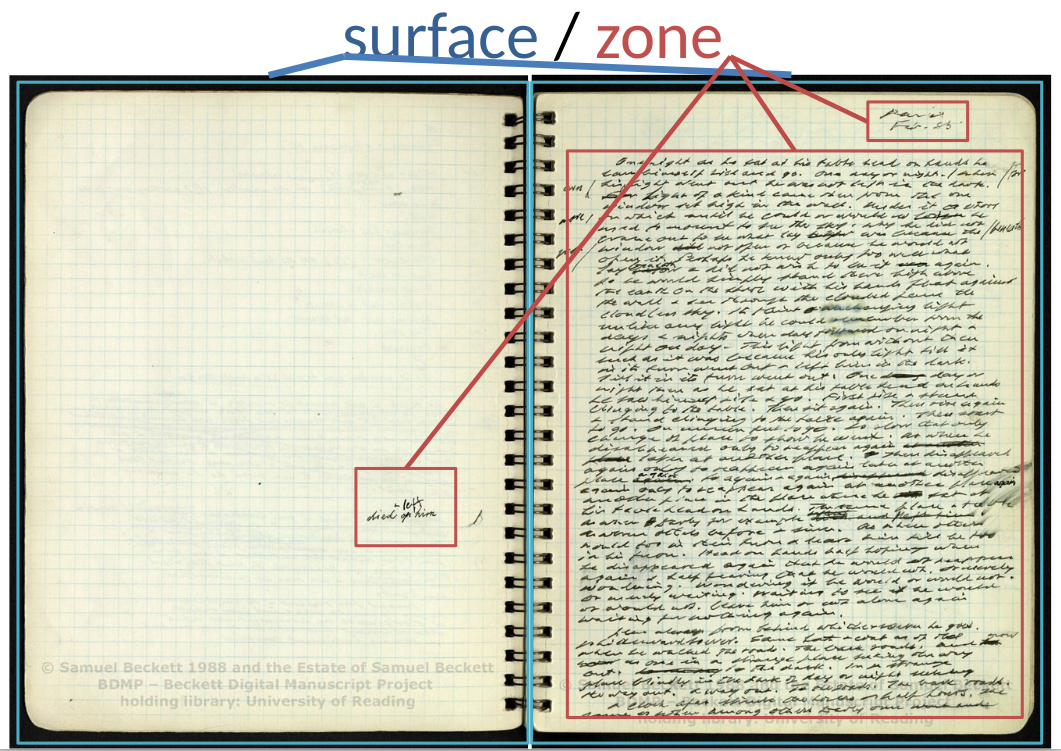
\includegraphics[width=\textwidth]{img/facs6.png}

\column{0.48\textwidth}
\begin{block}{Tools for text-image linking}
\begin{enumerate}\footnotesize
\item  \textbf{Image markup tool} (Martin Holmes, \protect\url{http://www.tapor.uvic.ca/~mholmes/image_markup/index.php})
\item  \textbf{TextGridLab:} http://www.textgridlab.de
\item  \textbf{T-PEN} (\protect\url{http://www.t-pen.org})
%\item  Faust-Edition: \protect\url{https://github.com/faustedition/ext-imageannotation}
\item \protect\url{http://imagecoordinates.com}
\end{enumerate}
\end{block}
\end{columns}

\framebreak


\begin{columns}
\column{0.48\textwidth}
\begin{block}{Embedded transcription}
\begin{itemize}\footnotesize
\item  "Embedded transcription": Text directly in \texttt{<surface>}
\item  \texttt{Relevant elements:} \texttt{<sourceDoc>}, \texttt{<surface>}, \texttt{<zone>}, \texttt{<line>}, \texttt{@rotate}
\end{itemize}
\end{block}

\column{0.48\textwidth}
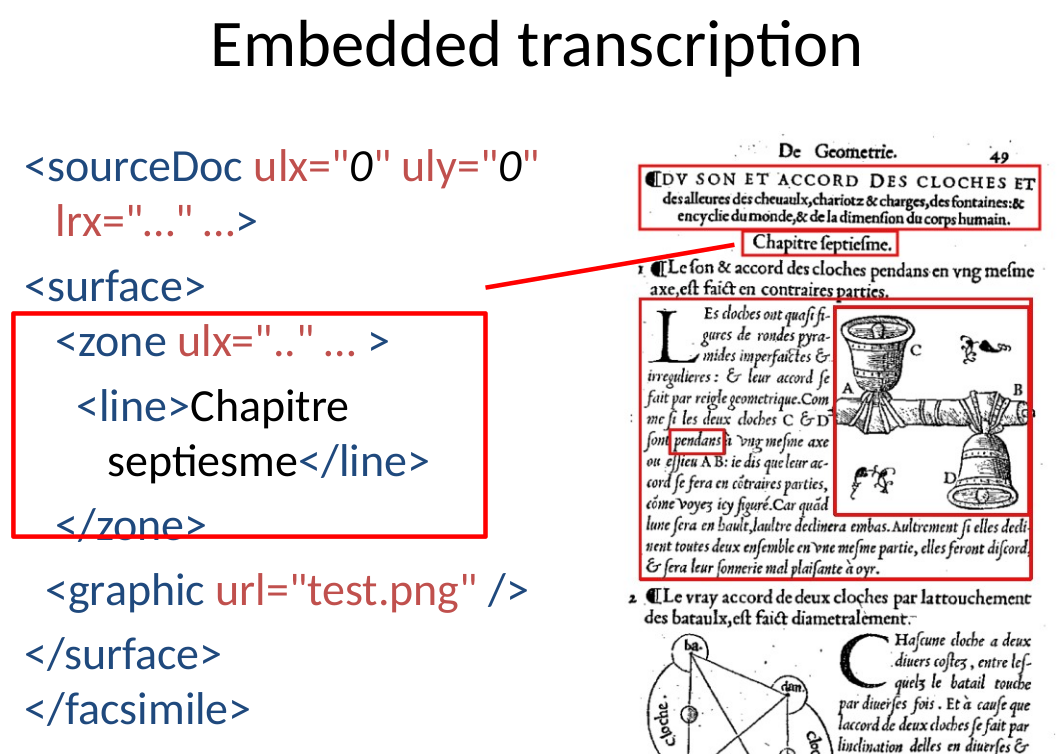
\includegraphics[width=\textwidth]{img/facs-embedded.png}
\end{columns}

\begin{xmlcode}
<sourceDoc>
 <surfaceGrp n="leaf1">
  <surface facs="page1.png"> <zone>All the writing on page 1</zone> </surface>
  <surface>
   <graphic url="page2-highRes.png"/>
   <zone> <line>A line of writing on page 2</line> </zone>
  </surface>
 </surfaceGrp>
</sourceDoc>
\end{xmlcode}

\end{frame}


%-----------------------------------------------------
\begin{frame}[allowframebreaks,fragile]{Critical Apparatus}
\subsubsection{Critical Apparatus in TEI}
\metroset{block=fill}
\dots aims at documenting the variants of a text in the witnesses of textual transmission.\medskip 

\begin{columns}
\column{0.48\textwidth}\small
A critical apparatus is encoded with:
\texttt{<app>}, \texttt{<rdg>} / \texttt{<rdgGrp>} and \texttt{<lem>}.
\texttt{<lem>} can contain text not documented in any textual witness.

\begin{xmlcode}
<app>
  <rdg wit="#Sh1">Then</rdg>
  <lem wit="#Sh2">Than</rdg>
</app> is my deede to my most  
<app>
  <lem wit="#Sh1">painted</rdg>
  <rdg wit="#Sh2">pained</rdg>
</app>word:

<app>
    <lem>deed</lem>
    <rdg wit="#Sh1 #Sh2">deede</rdg>
</app>
\end{xmlcode}

\column{0.48\textwidth}
\begin{xmlcode}
<app>
  <lem wit="#Sh2">Than</rdg>
  <rdg wit="#Sh1">Then</rdg>
</app> is my deede to my most  
<app>
  <lem wit="#Sh1">painted</rdg>
  <rdg wit="#Sh2">pained</rdg>
</app>word:

<app>
  <rdg wit="#Sh1">Then</rdg>
  <rdg wit="#Sh2">Than</rdg>
</app> is my deede to my most  
<app>
  <rdg wit="#Sh1">painted</rdg>
  <rdg wit="#Sh2">pained</rdg>
</app>word:
\end{xmlcode}

\end{columns}

\framebreak



\begin{columns}
\column{0.48\textwidth}\small 

The apparatus can be located anywhere as a \texttt{<listApp>}:
\begin{itemize}\footnotesize
    \item in the \texttt{<body>} of the document 
    \item in the \texttt{<back>} in other documents
    \item is referenced by \texttt{@loc}
\end{itemize}

$\to$ \texttt{<rdgGrp>} aggregates several readings of a common type.

\begin{block}{Witness list}
\texttt{@wit} refers to descriptions in the header: 
\texttt{<listWit>} = list of \texttt{<witness>}-elements identified by \texttt{@xml:id} each describing a textual witness e.g. by \texttt{<bibl>}- or \texttt{<msDesc>} elements in \texttt{teiHeader}/\texttt{sourceDesc}
\end{block}

\column{0.48\textwidth}
\begin{xmlcode}
<app>
    <rdgGrp type="orthographic">
        <rdg wit="#Sh1">giue</rdg>
        <rdg wit="#Sh2">give</rdg>
    </rdgGrp>
    <rdg wit="#AS1">have</rdg>
</app>

<listWit>
    <witness xml:id="Sh1">
  <bibl>Folger STC 22276</bibl>
    </witness>
    <witness xml:id="Sh2">
  <bibl>Huntington 69304</bibl>
    </witness>
</listWit>
\end{xmlcode}

\end{columns}

\framebreak


There are different options:
\begin{columns}
\column{0.48\textwidth}
\begin{block}{Location referenced + external}
\begin{xmlcode}
<p><pb n="f13"/><lb n="f13-z1" /> 
Dis ouentúrlich buoch bewiset wye 
von einer Frowen ge<lb/>nannt 
Melusina ...</p>
<!-- ... -->
<listApp><app loc="f13-z1">
    <lem wit="#BR1">ouentúrlich</lem>
    <rdg wit="#SK1">ouentuorlich</rdg>
    <rdg wit="#AS1">abenteürlich</rdg>
</app></listApp>
\end{xmlcode}
\end{block}



\column{0.48\textwidth}
\begin{block}{Double endpoint + external}\footnotesize

The apparatus is integrated into the \texttt{<body>} linked to identifiers for its beginning and its end (e.g. with \texttt{<anchor>}) but encoded anywhere (e.g. in the place where it was located in the printed source); referenced by \texttt{@from} \& \texttt{@to}.

\begin{xmlcode}
<p>Dis <anchor xml:id="A1"/>
ouentúrlich<anchor xml:id="A2"/> buoch
    bewiset wye von einer 
    Frowen ge<lb/>nannt Melusina 
    ...</p>
<!-- ... -->
<app from="#A1" to="#A2">
    <rdg wit="#SK1">ouentuorlich</rdg>
    <rdg wit="#AS1">abenteürlich</rdg>
</app>
\end{xmlcode}
\end{block}

\end{columns}

\framebreak

\begin{columns}
\column{0.48\textwidth}
\begin{block}{Location referenced + inline}
\begin{xmlcode}
<p n="p1">
    Dis ouentúrlich
    <app loc="p1">
        <rdg wit="#SK1">
           ouentuorlich</rdg>
        <rdg wit="#AS1">
           abenteürlich</rdg>
    </app>
    buoch bewiset wye 
    von einer Frowen 
    ge<lb/>nannt Melusina ...
</p>
\end{xmlcode}
\end{block}

\column{0.48\textwidth}

\begin{block}{Double endpoint + internal}\footnotesize
The apparatus is integrated into the \texttt{<body>} after the referenced passage and linked an identifiers for its beginning; referenced by \texttt{@from}.

\begin{xmlcode}
<p n="1">
    Dis <anchor xml:id="a"/>
    ouentúrlich<app from="#a">
        <rdg wit="#SK1">
           ouentuorlich</rdg>
        <rdg wit="#AS1">
           abenteürlich</rdg>
    </app>
    buoch bewiset wye von einer 
    Frowen ge<lb/>nannt Melusina
    ...
</p>
\end{xmlcode}
\end{block}
\end{columns}

\framebreak


\begin{columns}
\column{0.48\textwidth}
Last but not least\dots
\begin{block}{Parallel segmentation}\footnotesize
Encoding the „base text“ as the \texttt{lem} in the \texttt{app}-element. Can be done only inline. Possibility to nest variants.

\begin{xmlcode}
<p n="1">Dis
    <app>
        <lem wit="#BR1">
           ouentúrlich</lem>
        <rdg wit="#SK1">
           ouentuorlich</rdg>
        <rdg wit="#AS1">
           abenteürlich</rdg>
    </app>
    buoch bewiset wye von einer 
    Frowen ge<lb/>nannt Melusina
    ...
</p>
\end{xmlcode}
\end{block}

\column{0.48\textwidth}
\begin{block}{Which one to choose?}
\begin{enumerate}\footnotesize
    \item \textbf{Referenced} imitates the classical print version, is relatively fast to create but can be imprecise in referencing
    \item \textbf{Double-Endpoint} is relatively complex to encode and to process, but exact and the only form to handle overlapping structures
    \item \textbf{Parallel Segmentation} can be easily processed with XSLT but not very flexible in documenting complex changes and overlapping structures
\end{enumerate}
\end{block}
\end{columns}


\end{frame}

%-----------------------------------------------------
\begin{frame}[fragile]{Further suggestions}
\subsubsection{Suggestions for typical problems}
\metroset{block=fill}

\begin{columns}
\column{0.48\textwidth}
\begin{alertblock}{Suggestions for typical problems in editing}\footnotesize
\begin{description}
\item[Missing text (om.)] \texttt{<rdg>} remains empty; \texttt{@cause} can contain a controlled term to describe the situation (e.g. omisit)
\item[Additions (add.)] \texttt{<lem>} remains empty
\item[Corrections (corr. ex \dots)] \texttt{<rdg>} constains the complete encoding 
\end{description}
\end{alertblock}

\begin{xmlcode}
<subst><del>…</del><add>…</add></subst>
\end{xmlcode}

\column{0.49\textwidth}\scriptsize
\begin{block}{Tools for collation}
\begin{description}
\item[Juxta Commons] Texts are reduced to flat text. Variants are encoded in the parallel segmentation method.
\item[CollateX] Creates a graph. Compares every version with the existing graph and searches for gaps.
\end{description}
\end{block}

\begin{alertblock}{Stemmatology in TEI}
\begin{description}\scriptsize
\item[<eTree>]  each part of the tree which can have descendants
\item[<eLeaf>]  each part of the tree, which has only ancestors
\item[@type]  e.g. hypothetical, extant, lost \dots
\item[<label>]  for the short names („Sigla“)
\item[<ptr>]  for „contaminations“ i.e. texts influenced by other manuscript traditions
\end{description}
\end{alertblock}
\end{columns}


\end{frame}



%------------------------------------

\begin{frame}{TEI Critical Apparatus Toolbox}

    \begin{itemize}\small 
        \item \protect\url{http://teicat.huma-num.fr/}
        \item by Marjorie Burghart
        \item \textbf{Check encoding:} consistency etc.
        \item \textbf{Display parallel versions.}
        \item \textbf{Print an edition of a TEI XML edition,} with a TEI-to-\LaTeX{} and PDF transformation (\texttt{reledmac}! $\to$ \href{https://github.com/MarjorieBurghart/TEI-CAT/blob/master/tei2latex_final.xslt}{XSL is here}).
        \item \textbf{Annotate images:} lets you easily trace zones on an image to prepare a documentary edition (sometimes kind of buggy) $\to$ create your \texttt{<facsimile>}.
        \item \textbf{Get statistics} on the XML tags used in different parts of your edition plus word counts.
    \end{itemize}
    
    
\includegraphics[width=\textwidth]{img/tei-critical-app-toolbox.png}
\end{frame}



